\documentclass{article}
\usepackage[utf8]{inputenc}
\usepackage{tikz}
\usepackage{verbatim}
\documentclass[tikz,margin=2mm]{standalone}
\usetikzlibrary{trees,arrows}

\title{TP2-IFT3913}
\author{Wenhao Xu, 20150702\\Manping Li, 968527}
\date{}


\begin{document}

\maketitle

\section*{Tâche 1}

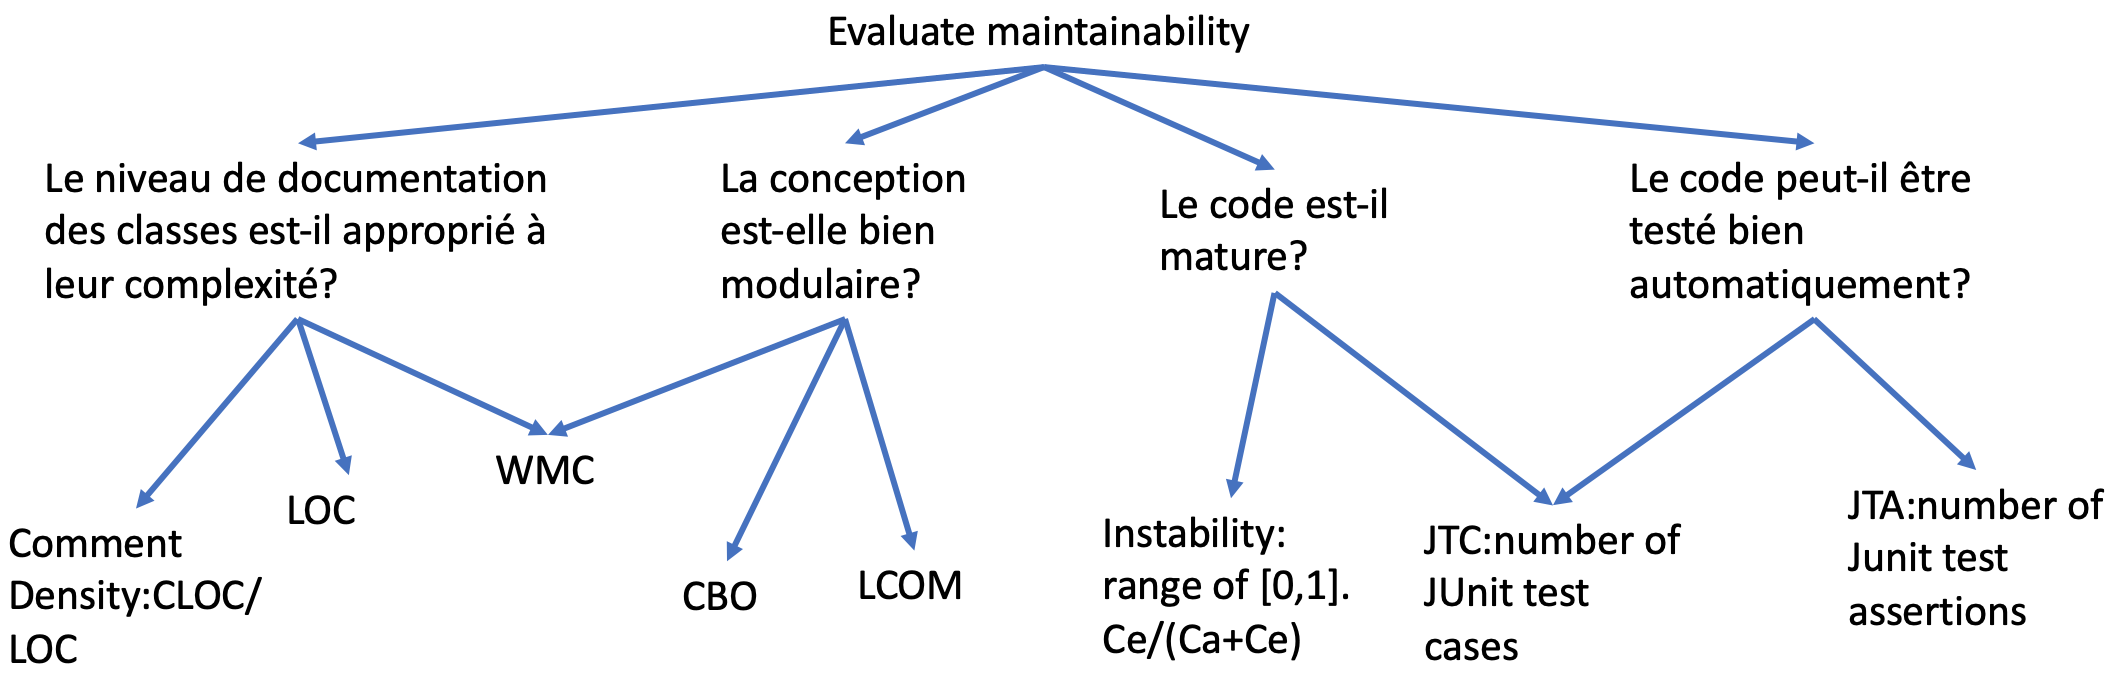
\includegraphics[width=0.95\textwidth]{GQM.png}\\\\
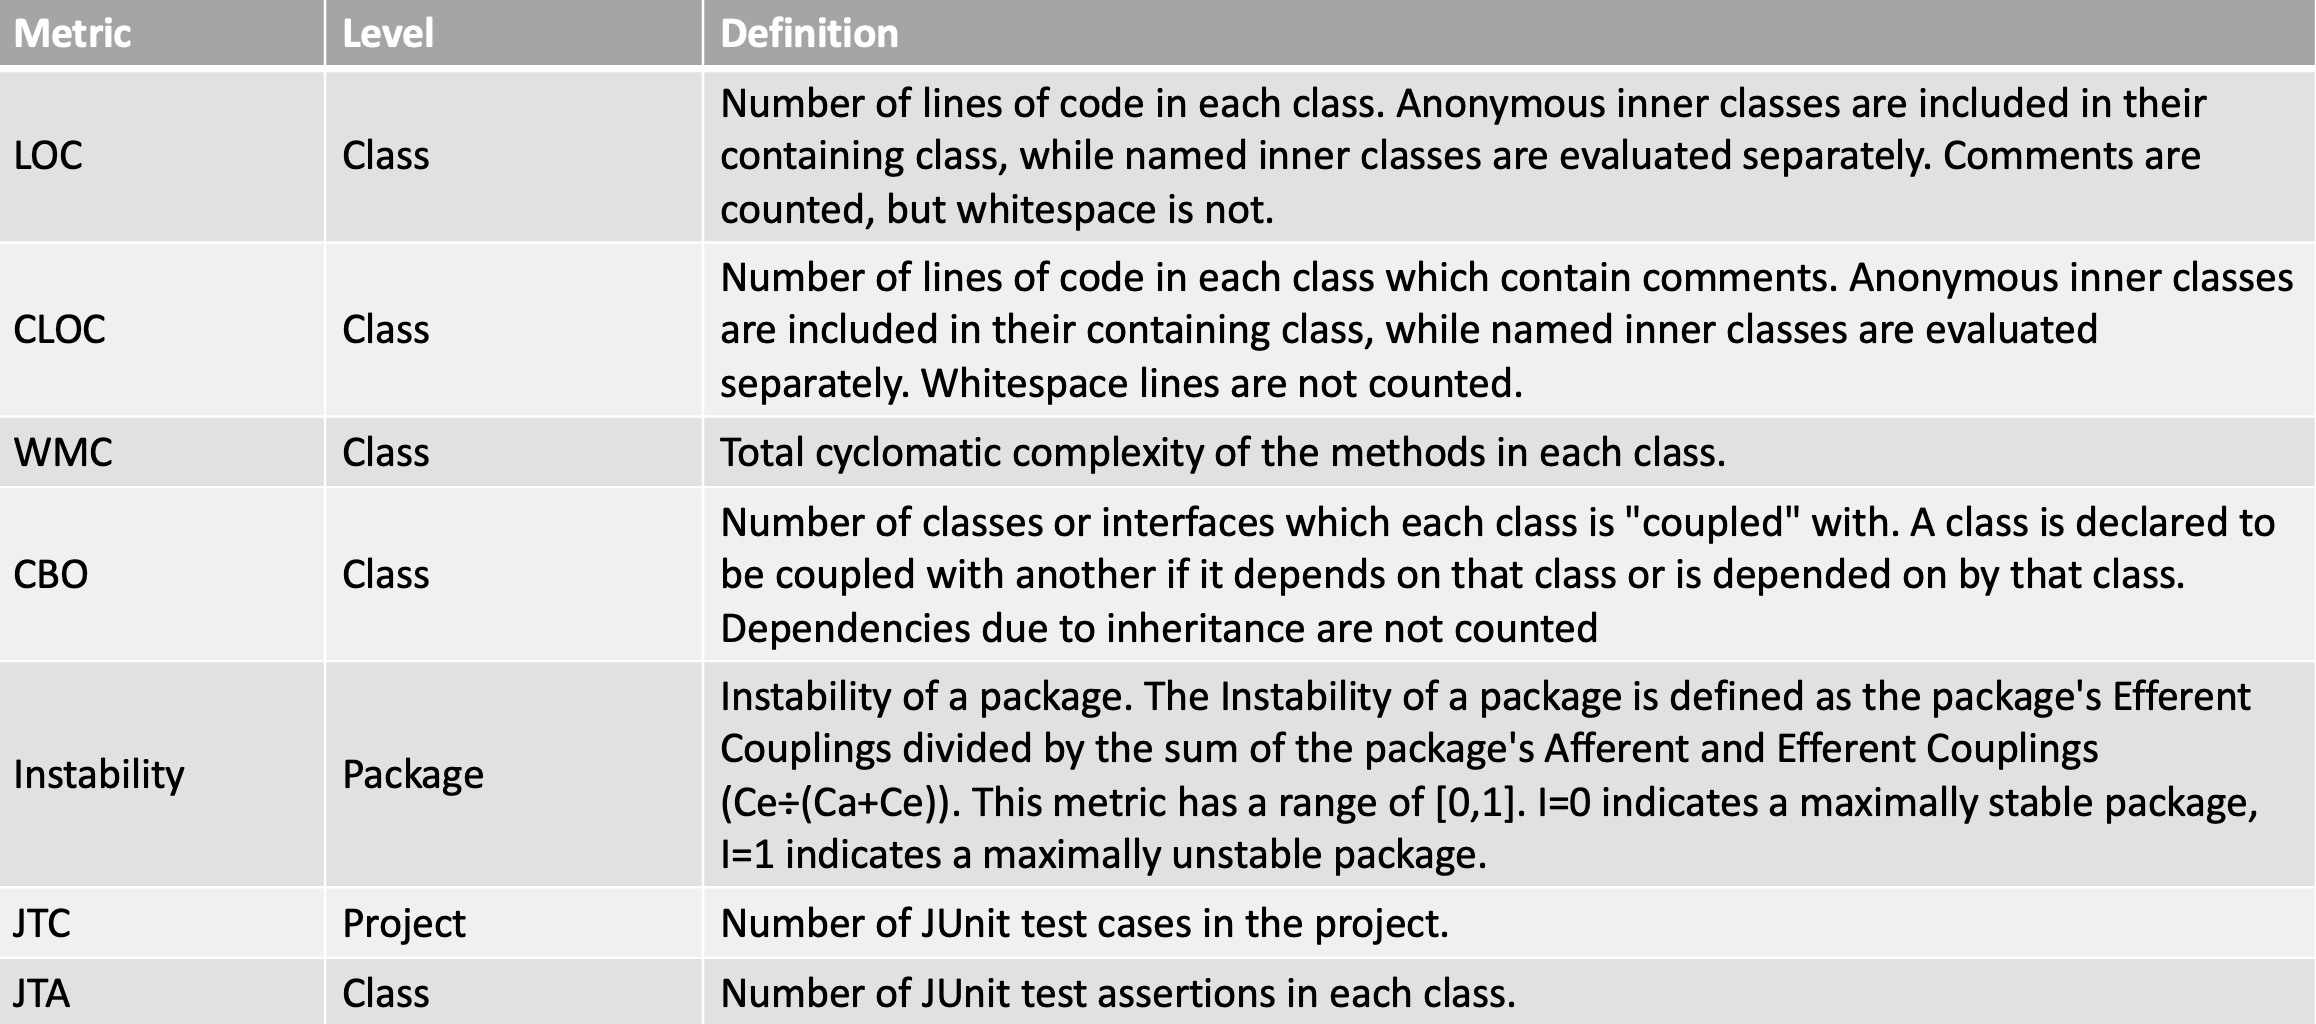
\includegraphics[width=0.95\textwidth]{Defi.png}\cite{ref 1 }\\\\
LOC\\
- We are using the metric LOC as it's well know as a software metric used to measure the size of a computer program by counting the number of lines in the text of the program's source code.\\
CLOC\\
- By mesuring CLOC, we take fully use to get the result of CLOC/LOC, the comment density. We believe that if a class has a proper complexity, it should has a proper comment density as well.\\
WMC\\
- If a class is well modularized and has a proper complexity, than the result of Weighted Methods Counts should be at a proper number, in which case, no too high.\\
CBO\\
- To reach a good modularity, the Coupling between objects should be low. Otherwise if one class depends or is depended too much on another case. Things often turn to be horrible when it comes to modification.\\
Instability\\
-\\
JTC\\
- A mature program should be simulated and tested for a wide range of possible error scenarios.\\
JTA

\section*{Tâche 2}
After trying various Metrics testers, we finally settled on Intellij's plugin MetricsReloaded as our test program. Not only is it very comprehensive in terms of the metrics it tests, but it is also easy to install and use.

\section*{Tâche 3}

\begin{thebibliography}{}  
 
     \bibitem{ref 1 }
 
       Powered by MetricsReloaded
 
\end{thebibliography}

% \tikzstyle{level 1}=[level distance=30mm, sibling distance=30mm]
% \tikzstyle{level 2}=[level distance=30mm, sibling distance=15mm]
% \tikzstyle{level 3}=[level distance=20mm]
% \begin{tikzpicture}[grow=right,->,>=angle 40]
% \begin{scope}[yshift=-6cm]
%   \node {Maintenabilité}
%     child {node {Q4}
%       child {node {Metric2}
%         child[-] {node{raison}}  
%       }
%       child {node {Metric1}
%         child[-] {node{raison}}  
%       }
%     }
%     child {node {Q3}
%       child {node {Metric2}
%         child[-] {node{raison}}  
%       }
%       child {node {Metric1}
%         child[-] {node{raison}}  
%       }
%     }
%     child {node {Q2}
%       child {node {Metric2}
%         child[-] {node{raison}}  
%       }
%       child {node {Metric1}
%         child[-] {node{raison}}  
%       }
%     }
%     child {node {Q1\footnotemark}
%       child {node {Metric2}
%         child[-] {node{raison}}  
%       }
%       child {node {Metric1}
%         child[-] {node{raison}}  
%       }
%     };
% \end{scope}
% \end{tikzpicture}


% \footnotetext{Q1 : Le niveau de documentation des classes est-il approprié par rapport à leur complexité ?, Q2 : La conception est-elle bien modulaire ?, Q3 : Le code est-il mature ?, Q4 : Le code peut-il être testé bien automatiquement ?}

% \begin{tikzpicture}   %创建环境
%     [thick,scale=0.8, every node/.style={scale=0.5}]
%     %thick,scale是整张树形图的大小,可以在0~1内调整树形图的大小
%     %every node/.style={scale=0.8}是每个节点文字的大小,可以修改调整节点文字的大小。
 
%     \node {Maintenabilité}
%     child {node {Q1 : Le niveau de documentation des classes est-il approprié par rapport à leur complexité ?}
%         child {node {树形架构}
%         }
%         child [missing] {}
%         child {node {平坦架构}
%         }
%         child [missing] {}
%         child {node {非结构型架构}
%         }
%     }    
%     child [missing] {}    %child [missing] {}充当间隔符号,隔开各个子树,可以增减其个数调整子树间距。
%     child [missing] {}
%     child [missing] {}       
%     child { node {Q2 : La conception est-elle bien modulaire ?}
%         child {node {巨型网络架构}
%         }
%         child [missing] {} %child [missing] {}充当间隔符号
%         child {node {标准网络架构}
%         }
%     }    
%     child [missing] {}
%     child [missing] {}    
%     child [missing] {}    
%     child { node {Q3 : Le code est-il mature ?}
%         child {node {无线网络架构}
%         }
%         child [missing] {}
%         child {node {光纤网络架构}
%         }
%     }
%     child [missing] {}    
%     child [missing] {} 
%     child { node {Q4 : Le code peut-il être testé bien automatiquement ?}
%         child {node {无线网络架构}
%         }
%         child [missing] {}
%         child {node {光纤网络架构}
%         }
%     }
%     ;
% \end{tikzpicture}

\end{document}
